%% ---------------------------------------------------------------------------
%% proposal.tex
%%
%% Research Proposal, main document.
%%
%% ---------------------------------------------------------------------------
\documentclass[12pt,letterpaper]{article}
\usepackage[english]{babel}     % supports english, but default is
% \usepackage[spanish]{babel}
% include this if you want to import graphics files with /includegraphics

\usepackage{longtable}
\usepackage{ifpdf}
\usepackage[table]{xcolor}

\usepackage{anysize}
\marginsize{2.5cm}{2.5cm}{1cm}{1cm}
\usepackage{textcomp}
\usepackage{url}
\bibliographystyle{unsrt}
\usepackage{graphics}
\usepackage{amssymb}
\usepackage{graphicx}
%\usepackage{slashbox}
\usepackage[latin1]{inputenc}
\usepackage{tikz}
\usetikzlibrary{arrows,positioning}
% Color and strikethrough

\usetikzlibrary{decorations.pathmorphing}
\usepackage{eso-pic}


\usepackage{color}
\usepackage{soul}

\usepackage{array}
\usepackage{makecell}

\usepackage{sectsty}
\allsectionsfont{\sffamily}

\definecolor{dblue}{RGB}{0,102,153}
\newcommand{\dB}[1]{\textcolor{dblue}{\textbf{#1}}}



\setlength{\parskip}{1em}

% Nombre del Estudiante
\newcommand{\scriptAuthor}{Daniel Moya S�nchez}

% T��tulo de la tesis
\newcommand{\scriptTitle}{Design Document v1} 


% Keywords
\newcommand{\scriptKeywords}{key, words, ...}

% Para el PDF (cambiar si se desea otras cosas a lo indicado arriba
\newcommand{\pdfAuthor}{\scriptAuthor}
\newcommand{\pdfTitle}{\scriptTitle} 
\newcommand{\pdfKeywords}{\scriptKeywords}


\tikzset{
    mynode/.style={rectangle,rounded corners,draw=black, top color=white, bottom color=yellow!50,very thick, inner sep=1em, minimum size=3em, text centered},
    myarrow/.style={->, >=latex', shorten >=1pt, thick},
    mylabel/.style={text width=7em, text centered} 
} 

\begin{document}
 
 \graphicspath{{./}{./fig/}}

 %% ---------------------------------------------------------------------------
%% titlepage.tex
%%
%% Title page
%%
%% ---------------------------------------------------------------------------

\thispagestyle{empty} 

\begin{center}

\textsc{\LARGE Instituto Tecnol\'ogico de Costa Rica} \\
\textsc{\Large Computer Engineering Academic Area}

\textsc{\Large Proyecto de Dise\~no en Ingenier\'ia en Computadores}


\par\vspace{20mm}

\includegraphics[scale=0.25]{logoTEC}

\par\vspace*{\fill}

{\LARGE\bf{\textsf{ \Huge \scriptTitle}}}

\par\vspace*{\fill}

%Master Thesis {\sf Proposal} \\ 
%in fulfillment of the requirements for the degree of
%Plan de Proyecto
%Master of Science in Electronics Engineering \\
%Emphasis on Embedded Systems

%\par\vspace{20mm}

\textsc{\Large \scriptAuthor}

\vspace*{\fill}

{\today}

\end{center}
\newpage 
\cleardoublepage  


%  \tableofcontents

 \clearpage
 
 \begin{table}[h!]
\begin{center}
\caption{Revision History}
\begin{tabular}{ | c | c | c | c | } 
 \hline
\textbf{Date}	&\textbf{Version}	&\textbf{Description}	&\textbf{Author} \\ \hline
02 March 2018	&1.0			&\makecell{Design Document for Design of \\  (ASIPs) for Approximate Computing}	&Daniel Moya \\ \hline
\end{tabular}
\label{tab:act}
\end{center}
\end{table}



\section{Introduction}



\subsection{Purpose}
The primary purpose of this document is to present a description of the design elements
of an ASIP in a general approximate application. 



\subsection{Scope}
This research concerns the selection and optimization of error-tolerant applications. For 
this, ASIP configurations using specific approximate instructions for the selected 
applications are to be delivered. Furthermore, each ASIP configuration will be described by 
a set of parameters that the final system will possess, such as energy efficiency, area, 
execution time, and output error. This project is expected to help approximate computing 
to be a more widespread tendency and generate a strong base knowledge for future 
projects where there is freedom to choose the parameters of hardware running a 
certain type of application in terms of resource consumption and accepted error. 



% Systems services and users
% Black Bow Design diagrams

% Entities: Actors, stakeholders, case uses

% Relationships: Output and input between actors and design

% constraints: QoS, form and medium of interaction
\subsection{Context}

Since approximated computing is still in its infancy, a lot of research and testing is still needed, 
so the users of the developed ASIPs are the same research groups behind this
project. \\

Figure \ref{fig:cont} shows the general scheme for an approximate possible application.

\begin{figure}[h!]
\centering
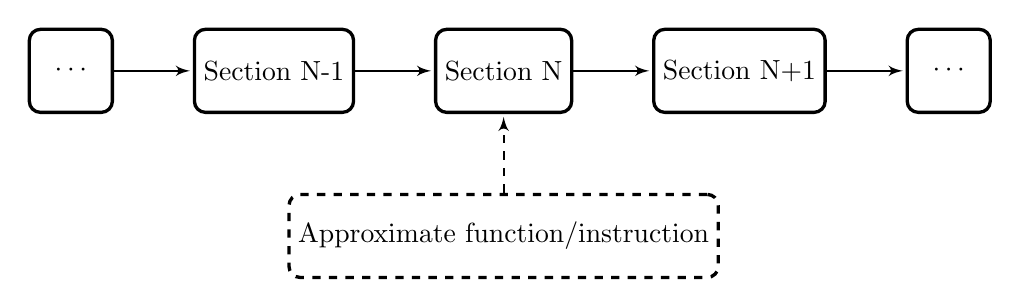
\begin{tikzpicture}[node distance=1cm, auto]  
\tikzset{
    mynode/.style={rectangle,rounded corners,draw=black, very thick, minimum size=3em, text centered},
    myarrow/.style={->, >=latex', shorten >=1pt, thick},
}
\node[mynode] (dots1) {$\cdots$};  
\node[mynode, right =1cm of dots1 ] (section1) {Section N-1};  
\node[mynode, right =1cm of section1] (section2) {Section N}; 
\node[mynode, right =1cm of section2] (section3) {Section N+1};
\node[mynode, right =1cm of section3] (dots2) {$\cdots$};  

\node[mynode, below=1cm of section2, dashed] (comment1) {Approximate function/instruction};

\draw[myarrow] (dots1.east)  ->  (section1.west);
\draw[myarrow] (section1.east)  ->  (section2.west);
\draw[myarrow] (section2.east)  ->  (section3.west);
\draw[myarrow] (section3.east)  ->  (dots2.west);

\draw[->, >=latex', shorten >=1pt, thick, dashed]  (comment1.north) -|  (section2.south); 
 
\end{tikzpicture} 
\medskip
\caption{General context of the application.} 
\label{fig:cont}
\end{figure}


As shown in figure \ref{fig:cont}, the approximate application is expected to have a pipeline structure, where one of its stages or sections (in that case
the n-th stage) can be approximate. The purpose of the ASIP configuration is to provide the user flexibility between
the original version of an application and the optimized one, allowing for a customized
balance between resource consumption and output error. The approximate section needs to perform the original action but with less resource consumption, and
still allowing for a acceptable output error, considering that a quality change in a specific section can have a big impact on other sections
that depend of it. 


\subsection{Summary}






% Referencias del Background y el Related Work
\bibliographystyle{sty/plainurl}
\bibliography{references}


\section{Glossary}


\begin{table}[h!]
\begin{center}
\caption{Definitions}
\begin{tabular}{|c|c|} 
 \hline
 Term & Definition \\ \hline
 ASIP & \makecell{
 Application Specific Instruction Set Processor. This means that, although the \\
 processor can execute a wide range of applications, it is optimized for a specific \\
 one, in which it can execute with improved performance (for instance, energy \\
 consumption or execution time would be lower) compared to a General Purpose \\
 Proccesor (GPP).}  \\ \hline
  GPP & \makecell{
 General Purpose Proccesor. In general, they show better flexibility than ASIPs \\
 because all the programs are executed in general-purpose components, but since \\
 they are not optimized, they show less resource efficiency.}  \\ \hline
   ASIC & \makecell{
 Application Specific Integrated Circuit. In general, they show better performance \\
results than ASIPs, nevertheless, they are less flexible when executing anything \\
other than the specific application they are meant to.}  \\ \hline
 ITCR & \makecell{
 Instituto Tecnol�gico de Costa Rica. Place from where this project is being \\
 developed.}  \\ \hline
\end{tabular}
\label{tab:def}
\end{center}
\end{table}



% Composition and modular assembly of
% systems in terms of subsystems and
% (pluggable) components, buy vs. build,
% reuse of components

% Entities: types of constituents of a system: subsystems, components, modules; ports and (provided
% and required) interfaces; also libraries, frameworks, software repositories, catalogs, and templates.

% Relationships: composition, use, and generalization

% Attributes: identification, type, purpose, function, and definition attribute should be utilized.
\section{Composition}

The ASIP configurations that will be developed are expected to impact on the Instruction Set Architecture (ISA)
and the processor components. For example, an assembly instruction may be created to be equivalent of two
other assembly instructions, with added hardware but less execution time, given that such operation is very frequent
on the high level program. Figure \ref{fig:comp} shows a general scheme for the interaction between these layers. 


\begin{figure}[h!]
\centering
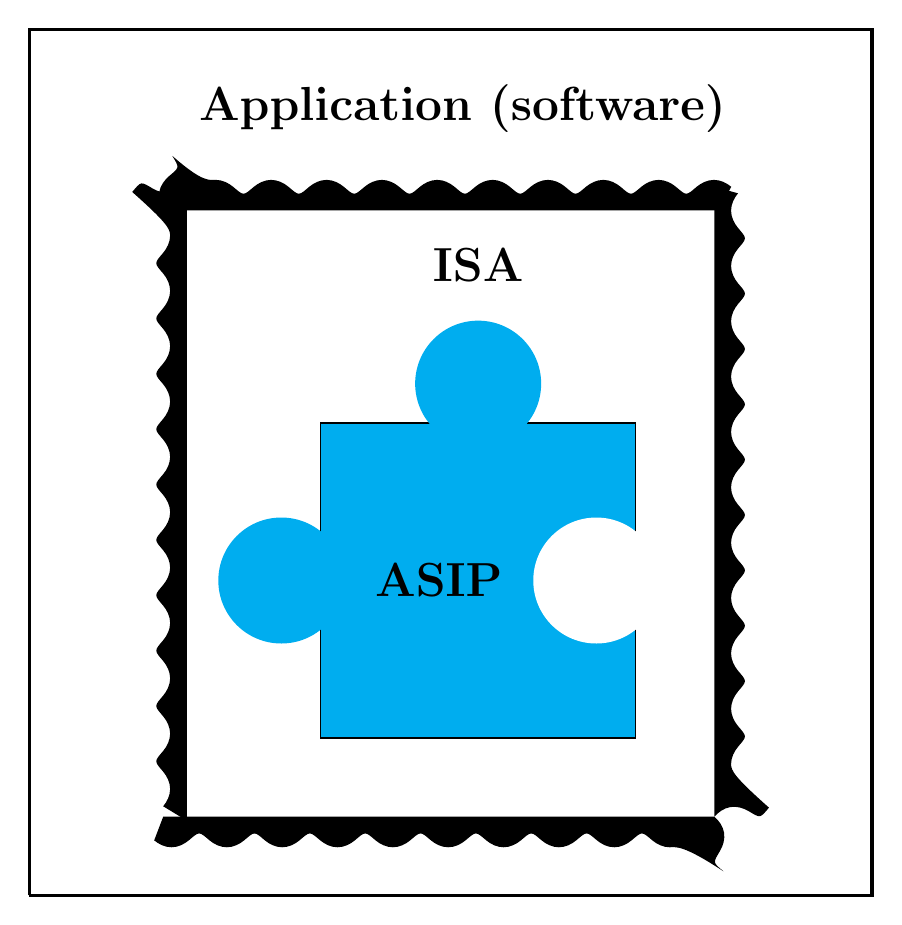
\begin{tikzpicture}[node distance=1cm, auto]  

\draw[fill=cyan] (7,1) -- (11,1) -- (11,5) -- (7,5) -- cycle;
\draw[fill=white,  draw=none](10.5,3) circle (.8cm);
\draw[fill=cyan,  draw=none](6.5,3) circle (.8cm);

\draw[fill=cyan, draw=none](9,5.5) circle (.8cm);
 
\node[] at (8.5,3) {\textbf{\LARGE{ASIP}}}; 


  \fill[black, decorate, decoration={coil,segment length=20pt}]     
    ([xshift=3mm,yshift=.5mm]5,8) --
    (5,8) --     
    (5,0) --
    ([xshift=3mm,yshift=-.5mm]5,0) ;
    
    
   \fill[black, decorate, decoration={coil,segment length=20pt}]
   (5,7.7) -- 
   ([xshift=.5mm,yshift=3mm]5,7.7) --      
   (12,8) --
   ([xshift=.5mm,yshift=-3mm]12,8) ;
   
   \fill[black, decorate, decoration={coil,segment length=20pt}]
   (12,0) -- 
   ([xshift=3mm,yshift=.5mm]12,0) --  
   ([xshift=3mm,yshift=-.5mm]12,8) --
   (12,8) ;
   
   \fill[black, decorate, decoration={coil,segment length=20pt}]
   (12,0) -- 
   ([xshift=.5mm,yshift=-3mm]12,0) --  
   ([xshift=.5mm,yshift=-3mm]5,0) --
   (5,0) ;
         
\node[] at (9,7) {\textbf{\LARGE{ISA}}}; 

   \draw[very thick] (3.3,-1) -- (3.3,10) -- (14,10) -- (14,-1) -- (3.3,-1) ;
   
\node[] at (8.8,9) {\textbf{\LARGE{Application (software)}}};
 
\end{tikzpicture} 
\medskip
\caption{Componnent} 
\label{fig:comp}
\end{figure}


% Static structure (classes, interfaces, and
% their relationships)
% Reuse of types and implementations
% (classes, data types)

%  classes and interfaces with their structural stabuttic relationshipsstances of types in outlining design ideas.
\section{Logical}
Since the selected application is not going to be altered, this section does not apply.  

% Interconnection, sharing, and
% parameterization

% The Dependency viewpoint specifies the relationships of interconnection and access among entities. These
% relationships include shared information, order of execution, or parameterization of interfaces.
\section{Dependency}
The approximate functions or instructions are expected to have to retain the original dependencies in a specific application. 


%Information with data
% distribution overlay and physical
% volumetric overlay
% Persistent information

% Entities: data items, data types and classes, data stores, and access mechanisms.
% Relationships: association, uses, implements. Data attributes, their constraints and static
% relationships among data entities, aggregates of attributes, and relationships.
% Attributes: persistence and quality properties.
\section{Information}
This section does not apply.

% Reuse of patterns and available
% Framework template

% Key concerns include reuse at the level of design ideas (design patterns), architectural styles, and
% framework templates.
\section{Patterns}
This section does not apply. 

% Service definition, service access

%External and internal interfaces (NOT GUI)
\section{Interfaces}
This section does not apply. 

%Service definition, service access
\subsection{User interface}
Since the actual results of this research is knowledge, no user interface is made.

% Internal constituents and organization of
% design subjects, components and classes

% Compositional structure of coarse-grained components and reuse of fine-grained components.
\section{Structure}
The hardware structure of the generated ASIPs will consist of the usual components for a pipeline
processor (e.g ALU, registers) but with additional specialized components (according to the application)
and reduced generic hardware (e.g ALU may only have needed operations).

% The Interaction viewpoint defines strategies for interaction among entities, regarding why, where, how, and
% at what level actions occur.
\section{Interaction}
The interaction between the hardware components will follow a general pipeline scheme.


% System dynamics including modes, states, transitions, and reactions to events.
\section{State dynamics}
This section does not apply-

% The detailed design description of operations (such as methods and functions), the internal details and logic
% of each design entity.
\section{Algorithm}
This section does not apply.

% The purpose of the Resource viewpoint is to model the characteristics and utilization of resources in a
% design subject.
\section{Resources}
Since the resources consumption in an approximate application is one of this research's objetives topics, this section does not apply. 




\end{document}

